

\tikzset{every picture/.style={line width=0.75pt}} %set default line width to 0.75pt        

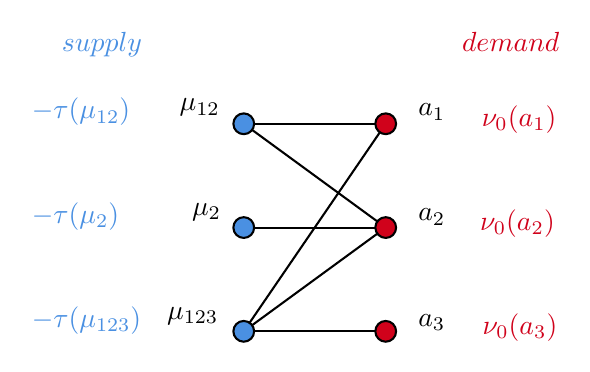
\begin{tikzpicture}[x=0.75pt,y=0.75pt,yscale=-1,xscale=1]
%uncomment if require: \path (0,300); %set diagram left start at 0, and has height of 300

%Straight Lines [id:da6692255227134147] 
\draw    (119.6,50.6) -- (188,50.6) ;
%Straight Lines [id:da17412111359948068] 
\draw    (119.6,50.6) -- (188,100.6) ;
%Straight Lines [id:da5786581212363588] 
\draw    (119.6,100.6) -- (188,100.6) ;
%Straight Lines [id:da5294359176796788] 
\draw    (119.6,150.6) -- (188,150.6) ;
%Straight Lines [id:da31575092120591086] 
\draw    (119.6,150.6) -- (188,100.6) ;
%Straight Lines [id:da23269865192852035] 
\draw    (119.6,150.6) -- (188,50.6) ;
%Shape: Circle [id:dp8181965387193857] 
\draw  [fill={rgb, 255:red, 74; green, 144; blue, 226 }  ,fill opacity=1 ] (114.6,50.6) .. controls (114.6,47.84) and (116.84,45.6) .. (119.6,45.6) .. controls (122.36,45.6) and (124.6,47.84) .. (124.6,50.6) .. controls (124.6,53.36) and (122.36,55.6) .. (119.6,55.6) .. controls (116.84,55.6) and (114.6,53.36) .. (114.6,50.6) -- cycle ;
%Shape: Circle [id:dp4767598139066547] 
\draw  [fill={rgb, 255:red, 74; green, 144; blue, 226 }  ,fill opacity=1 ] (114.6,100.6) .. controls (114.6,97.84) and (116.84,95.6) .. (119.6,95.6) .. controls (122.36,95.6) and (124.6,97.84) .. (124.6,100.6) .. controls (124.6,103.36) and (122.36,105.6) .. (119.6,105.6) .. controls (116.84,105.6) and (114.6,103.36) .. (114.6,100.6) -- cycle ;
%Shape: Circle [id:dp01302521130012857] 
\draw  [fill={rgb, 255:red, 74; green, 144; blue, 226 }  ,fill opacity=1 ] (114.6,150.6) .. controls (114.6,147.84) and (116.84,145.6) .. (119.6,145.6) .. controls (122.36,145.6) and (124.6,147.84) .. (124.6,150.6) .. controls (124.6,153.36) and (122.36,155.6) .. (119.6,155.6) .. controls (116.84,155.6) and (114.6,153.36) .. (114.6,150.6) -- cycle ;
%Shape: Circle [id:dp8977876171203294] 
\draw  [fill={rgb, 255:red, 208; green, 2; blue, 27 }  ,fill opacity=1 ] (183,50.6) .. controls (183,47.84) and (185.24,45.6) .. (188,45.6) .. controls (190.76,45.6) and (193,47.84) .. (193,50.6) .. controls (193,53.36) and (190.76,55.6) .. (188,55.6) .. controls (185.24,55.6) and (183,53.36) .. (183,50.6) -- cycle ;
%Shape: Circle [id:dp8770291086241786] 
\draw  [fill={rgb, 255:red, 208; green, 2; blue, 27 }  ,fill opacity=1 ] (183,100.6) .. controls (183,97.84) and (185.24,95.6) .. (188,95.6) .. controls (190.76,95.6) and (193,97.84) .. (193,100.6) .. controls (193,103.36) and (190.76,105.6) .. (188,105.6) .. controls (185.24,105.6) and (183,103.36) .. (183,100.6) -- cycle ;
%Shape: Circle [id:dp8383370432071702] 
\draw  [fill={rgb, 255:red, 208; green, 2; blue, 27 }  ,fill opacity=1 ] (183,150.6) .. controls (183,147.84) and (185.24,145.6) .. (188,145.6) .. controls (190.76,145.6) and (193,147.84) .. (193,150.6) .. controls (193,153.36) and (190.76,155.6) .. (188,155.6) .. controls (185.24,155.6) and (183,153.36) .. (183,150.6) -- cycle ;

% Text Node
\draw (93.2,87.4) node [anchor=north west][inner sep=0.75pt]    {$\mu _{2}$};
% Text Node
\draw (87.2,37.2) node [anchor=north west][inner sep=0.75pt]    {$\mu _{12}$};
% Text Node
\draw (81.2,137.6) node [anchor=north west][inner sep=0.75pt]    {$\mu _{123}$};
% Text Node
\draw (202.2,39.6) node [anchor=north west][inner sep=0.75pt]    {$a_{1}$};
% Text Node
\draw (202.2,90.2) node [anchor=north west][inner sep=0.75pt]    {$a_{2}$};
% Text Node
\draw (202.2,140.8) node [anchor=north west][inner sep=0.75pt]    {$a_{3}$};
% Text Node
\draw (232.8,40.4) node [anchor=north west][inner sep=0.75pt]  [color={rgb, 255:red, 208; green, 2; blue, 27 }  ,opacity=1 ]  {$\nu _{0}( a_{1})$};
% Text Node
\draw (232,90.5) node [anchor=north west][inner sep=0.75pt]  [color={rgb, 255:red, 208; green, 2; blue, 27 }  ,opacity=1 ]  {$\nu _{0}( a_{2})$};
% Text Node
\draw (233.2,140.6) node [anchor=north west][inner sep=0.75pt]  [color={rgb, 255:red, 208; green, 2; blue, 27 }  ,opacity=1 ]  {$\nu _{0}( a_{3})$};
% Text Node
\draw (16,36.8) node [anchor=north west][inner sep=0.75pt]  [color={rgb, 255:red, 74; green, 144; blue, 226 }  ,opacity=1 ]  {$-\tau ( \mu _{12})$};
% Text Node
\draw (16,87) node [anchor=north west][inner sep=0.75pt]  [color={rgb, 255:red, 74; green, 144; blue, 226 }  ,opacity=1 ]  {$-\tau ( \mu _{2})$};
% Text Node
\draw (16,137.2) node [anchor=north west][inner sep=0.75pt]  [color={rgb, 255:red, 74; green, 144; blue, 226 }  ,opacity=1 ]  {$-\tau ( \mu _{123})$};
% Text Node
\draw (30.5,4.8) node [anchor=north west][inner sep=0.75pt]  [color={rgb, 255:red, 74; green, 144; blue, 226 }  ,opacity=1 ]  {$supply$};
% Text Node
\draw (223.3,4.8) node [anchor=north west][inner sep=0.75pt]  [color={rgb, 255:red, 208; green, 2; blue, 27 }  ,opacity=1 ]  {$demand$};

\end{tikzpicture}